% \input{"IAB/latex/TeX-Folienformat.tex"}
\input{"/Users/jonathanlatner/Google Drive/My Drive/IAB/latex/TeX-Folienformat.tex"}

\documentclass[t,8pt,utfx8]{beamer}
\usepackage{booktabs}
\usepackage{setspace}
\usepackage{parskip}
\usepackage{graphicx}
\usepackage{subcaption}
\setbeamertemplate{caption}[numbered]
\newcommand{\sprache}{\englisch}
\renewcommand{\thesubsection}{\alph{subsection})}
\usepackage[cal=pxtx, scr=dutchcal]{mathalpha}
\usepackage{forest}



\definecolor{codegreen}{rgb}{0,0.6,0}
\definecolor{codegray}{rgb}{0.5,0.5,0.5}
\definecolor{codepurple}{rgb}{0.58,0,0.82}
\definecolor{backcolour}{rgb}{0.95,0.95,0.92}


\usepackage{listings}

% Define style for R code
\lstset{
  language=R,
  basicstyle=\ttfamily\small,
  keywordstyle=\color{blue},
  stringstyle=\color{red},
  commentstyle=\color{green},
  showstringspaces=false,
  numbers=left,
  numberstyle=\tiny\color{gray},
  stepnumber=1,
  numbersep=5pt,
  breaklines=true,
  frame=single
}

\newcommand{\btVFill}{\vskip0pt plus 1filll}


\title{Buyer Beware: Understanding the trade-off between utility and risk in CART based models using simulation data}

\subtitle{Berlin, \newline 7-8. Oktober, 2024}

\author{Jonathan Latner, PhD \newline Dr. Marcel Neuenhoeffer \newline Prof. Dr. Jörg Drechsler}

\newcounter{noauthorlines}
\setcounter{noauthorlines}{2} % Wert für 2 Autoren über 2 Zeilen. Ggf. anpassen

% %%%%%%%%%%%%%%
% Ende Anpassung
% %%%%%%%%%%%%%%

% \input{"IAB/latex/TeX-Folienformatierung_CD_2019"}
\input{"/Users/jonathanlatner/Google Drive/My Drive/IAB/latex/TeX-Folienformatierung_CD_2019"}

% Modify the section in toc template to enumerate
\setbeamertemplate{section in toc}{%
    \inserttocsectionnumber.~\inserttocsection\par
}

% use for subsections
% \setbeamertemplate{subsection in toc}{}
\setbeamertemplate{subsection in toc}{%
    \setlength{\parskip}{1mm}
        \hskip2mm -- \hskip1mm\inserttocsubsection\par
}


\usepackage{colortbl}
\definecolor{lightgray}{gray}{0.9}

\usepackage{listings} %include R code
\lstdefinestyle{mystyle}{
    backgroundcolor=\color{backcolour},   
    commentstyle=\color{codegreen},
    keywordstyle=\color{magenta},
    numberstyle=\tiny\color{codegray},
    stringstyle=\color{codepurple},
    basicstyle=\ttfamily\tiny,
    breakatwhitespace=false,         
    breaklines=true,                 
    captionpos=b,                    
    keepspaces=true,                 
    numbers=left,                    
    numbersep=5pt,                  
    showspaces=false,                
    showstringspaces=false,
    showtabs=false,                 
    columns=fullflexible,
    frame=single,
    tabsize=2
}
\lstset{style=mystyle}


\begin{document}


\frame[plain]{\titlepage}

\begin{spacing}{1.25}


%%%%%%%%%%%%%%%%%%%%%%%%%%%%%%%%%%%%%%%%
%%%%%%%%%%%%%%%%%%%%%%%%%%%%%%%%%%%%%%%%
\section{Introduction}\label{sec:introduction}
%%%%%%%%%%%%%%%%%%%%%%%%%%%%%%%%%%%%%%%%
%%%%%%%%%%%%%%%%%%%%%%%%%%%%%%%%%%%%%%%%

\begin{frame}[c,plain]
\vskip-4mm
\begin{beamercolorbox}[wd=\boxwidth,ht=22.11mm]{transparent}%
    \vfill%
    \usebeamerfont{title}%
    \leftinsert%
    \MakeUppercase{Section \ref{sec:introduction}: Introduction
} % <- Hier die Überschrift eintragen
\end{beamercolorbox}
\vskip-3mm
\pgfuseimage{rahmenlinie}
\end{frame}


\frame{\frametitle{Overview}
\begin{itemize}
    \item It is well established that there is a trade-off between utility and privacy when generating synthetic data
    \item Utility in CART based synthesizers is high (Little et al., 2022; Danker and Ibrahim, 2021)
    \item Privacy in CART based synthesizers is also high (Little et al., 2022)
    \item It seemed that CART models are less sensitive to this trade-off than other SDGs (i.e. higher utility, lower risk)
    \item Using simulation data (Reiter et al., 2014), results suggest synthetic data from CART models are disclosive
    \item Disclosive in ways that are not observable using traditional privacy measures
    \item It is possible to increase protection (by reducing utility), but you have to choose to do so
    \item More generally: If you did not know there was a problem, why would correct it?
\end{itemize}
}

\frame{\frametitle{Whats the goal of synthetic data?}
\begin{itemize}
    \item Synthetic data can accelerate development by replacing sensitive values with synthetic ones with minimal distortion of the statistical information contained in the original data set. (Jordan et al., 2022; Nowak et al., 2016)
    \item Low disclosure risk (R)
    \item High data utility (U)
    \item Visualize the trade-off using the R-U confidentiality map (Duncan et al., 2004)
\end{itemize}
}

\frame{\frametitle{Whats the problem?}
\begin{itemize}
    \item High data utility -- It must be similar to and different from the original data. 
    \begin{itemize}
        \item At the extreme, if the goal is high utility, why not just release the original data?
    \end{itemize}
    \item Low disclosure risk -- Synthetic data is not automatically private. 
    \begin{itemize}
        \item At the extreme, if the goal is low privacy risk, why should we release any data?
    \end{itemize}
    \item Many measures of utility and privacy exist
    \begin{itemize}
        \item Therefore, its not clear if data have high utility or low risk
        \item 2 problems
        \begin{itemize}
            \item More specifically, how can we map R-U trade-off if there are multiple measures of both?
            \item More generally, how do we know if the data have high levels of utility and low levels of privacy?
        \end{itemize}
    \end{itemize}
\end{itemize}
}


\frame{\frametitle{What do we know?}
\begin{itemize}
    \item Reiter (2005) suggested using sequential modeling with Classification and Regression Trees (CART). 
    \item Utility
    \begin{itemize}
        \item Drechsler and Reiter (2011) found that CART models offered the best results in terms of preserving the information from the original data.
        \item Other comparisons also found CART is superior (Little et al., 2022; Danker and Ibrahim, 2021)
    \end{itemize}
    \item Privacy
    \begin{itemize}
        \item Some evidence also suggests CART is superior (Little et al., 2022)
        \item However, other evidence indicates that CART-based synthesis simply replicates most of the original records (Manrique-Vallier and Hu, 2018)
    \end{itemize}
\end{itemize}
}

\frame{\frametitle{How does sequential modeling with CART work}
Nowak et al., 2022
\begin{itemize}
    \item Consider as an example a default synthesis, i.e. synthesis with all values of all variables ($Y_1, Y_2,\dots, Y_p$) to be replaced. 
    \item The first variable is generated by random sampling with replacement from its observed values. 
    \item The second variable to be synthesized ($Y_2$) is generated using the fitted model and the synthesised values of ($Y_1$). 
    \item The third variable to be synthesized ($Y_3$) is generated using the fitted model and the synthesized values of $Y_1$ and ($Y_2$)
    \item The distribution of the last variable ($Y_p$) will be conditional on all other variables. 
\end{itemize}
}

%%%%%%%%%%%%%%%%%%%%%%%%%%%%%%%%%%%%%%%%
%%%%%%%%%%%%%%%%%%%%%%%%%%%%%%%%%%%%%%%%
\section{Data and methods}\label{sec:data_methods}
%%%%%%%%%%%%%%%%%%%%%%%%%%%%%%%%%%%%%%%%
%%%%%%%%%%%%%%%%%%%%%%%%%%%%%%%%%%%%%%%%
\begin{frame}[c,plain]
\vskip-4mm
\begin{beamercolorbox}[wd=\boxwidth,ht=22.11mm]{transparent}%
    \vfill%
    \usebeamerfont{title}%
    \leftinsert%
    \MakeUppercase{Section \ref{sec:data_methods}: Data and methods
} % <- Hier die Überschrift eintragen
\end{beamercolorbox}
\vskip-3mm
\pgfuseimage{rahmenlinie}
\end{frame}


\frame{\frametitle{Data and methods}
\begin{itemize}
    \item Data - simulated data (Reiter et al., 2024)
    \item Utility measures (synthpop - Raab et al., 2021)
    \begin{itemize}
        \item Voas Williamson 
        \item Freeman-Tukey
        \item Jensen-Shannaon divergence
        \item Kolmogorov-Smirnov statistic
        \item Propensity score mean-squared error
        \item Bhattacharyya distances  
    \end{itemize}
    \item Privacy measures (synthpop - Raab et al., 2024)
    \begin{itemize}
        \item Identity disclosure measure
        \item Attribute disclosure measure
        \item Replicated uniques
    \end{itemize}
\end{itemize}
}


\frame{\frametitle{Simulate data with a unique record}

Borrowing from Reiter et al. (2014), we set the first 999 observations to be a random sample from a multinomial distribution for all combinations of $var1(0,1), var2(0,1), var3(0,1), var3(0,1)$ except (var1=1,var2=1,var3=1,var4=1), which we set to be the 1000th observation. 

\begin{minipage}{0.48\textwidth}
    \centering
    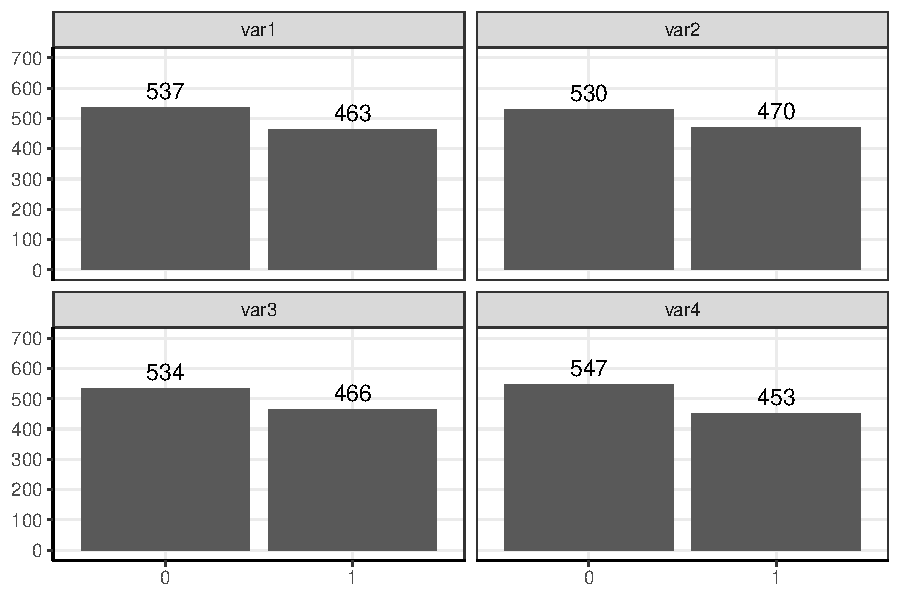
\includegraphics[width=\textwidth]{../../graphs/graph_numeric_frequency.pdf}
    \captionof{figure}{Frequency}
\end{minipage}
\hfill
\begin{minipage}{0.48\textwidth}
    \centering
    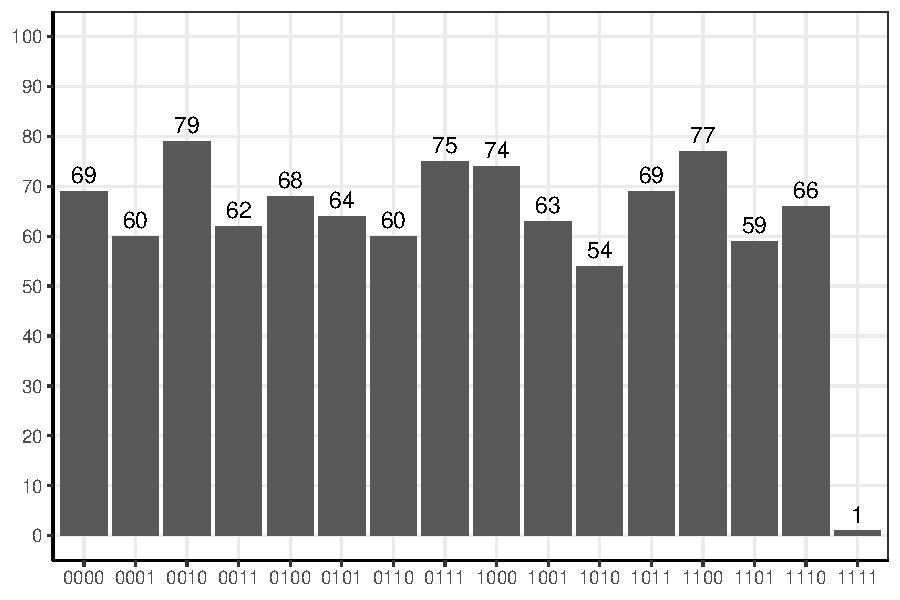
\includegraphics[width=\textwidth]{../../graphs/graph_numeric_histogram.pdf}
    \captionof{figure}{Histogram}
\end{minipage}

}

\frame{\frametitle{Simulate data with a unique record}

\begin{minipage}{0.48\textwidth}
    \centering
    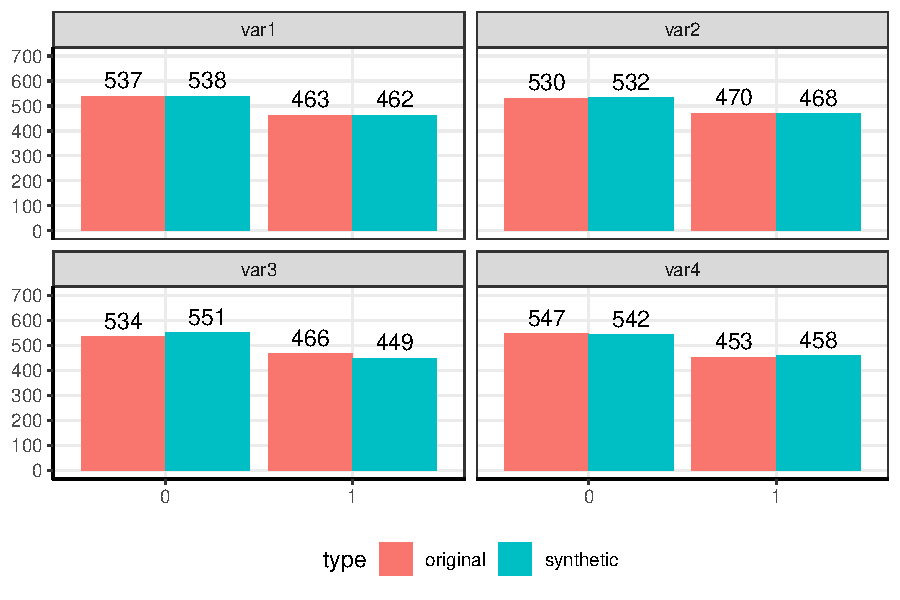
\includegraphics[width=\textwidth]{../../graphs/graph_numeric_compare_frequency.pdf}
    \captionof{figure}{Frequency}
\end{minipage}
\hfill
\begin{minipage}{0.48\textwidth}
    \centering
    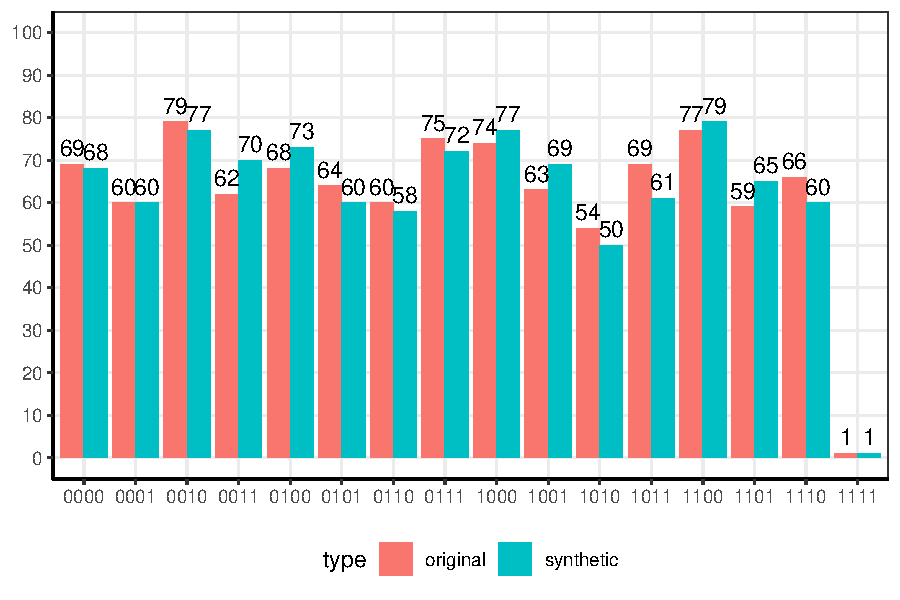
\includegraphics[width=\textwidth]{../../graphs/graph_numeric_compare_histogram.pdf}
    \captionof{figure}{Histogram}
\end{minipage}

}

\frame{\frametitle{Compare histogram x 100 synthetic datasets}
\begin{figure}
    \caption{}
    \resizebox{\textwidth}{!}{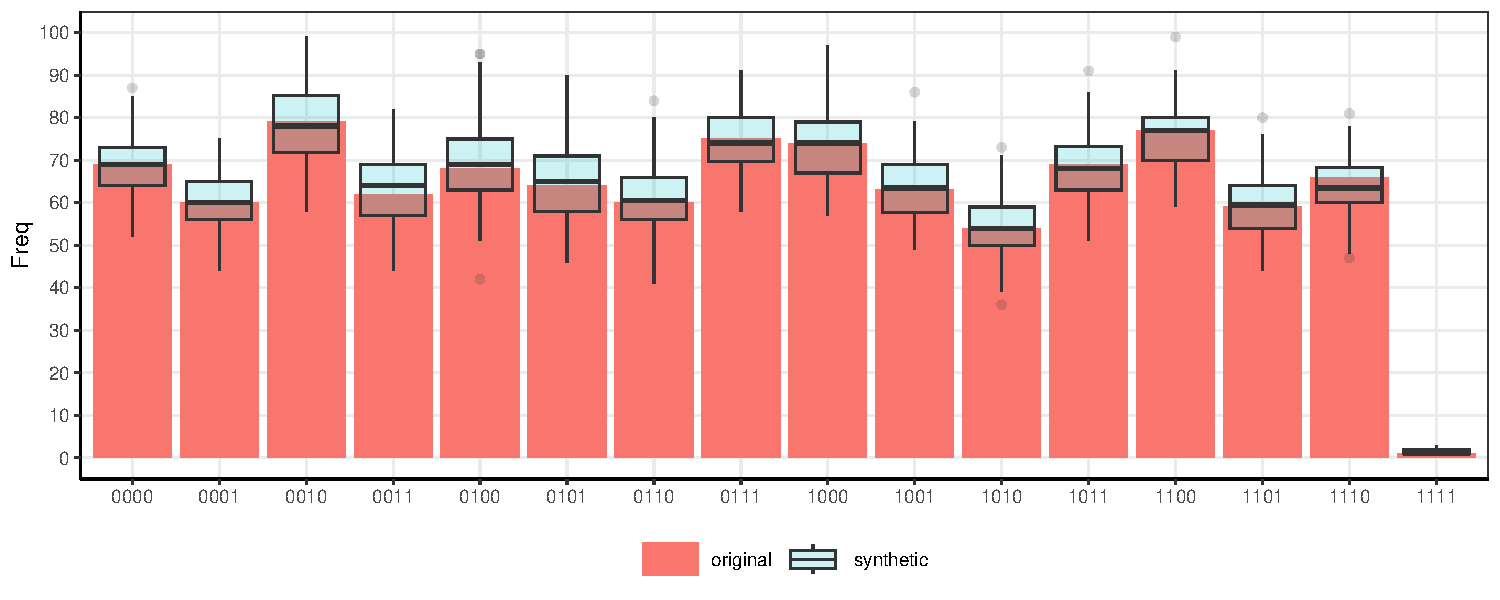
\includegraphics{../../graphs/graph_numeric_compare_histogram_100.pdf}}
    \label{fig:graph_numeric_compare_histogram_100}
\end{figure}
}

%%%%%%%%%%%%%%%%%%%%%%%%%%%%%%%%%%%%%%%%
%%%%%%%%%%%%%%%%%%%%%%%%%%%%%%%%%%%%%%%%
\section{Measuring utility and privacy}\label{sec:measuring}
%%%%%%%%%%%%%%%%%%%%%%%%%%%%%%%%%%%%%%%%
%%%%%%%%%%%%%%%%%%%%%%%%%%%%%%%%%%%%%%%%
\frame{\frametitle{Comparing utility measures}
\begin{table}[ht]
    \caption{}
    \centering
    \rowcolors{1}{white}{lightgray}
    \resizebox{\textwidth}{!}{% latex table generated in R 4.4.0 by xtable 1.8-4 package
% Mon Sep 30 14:13:42 2024
\begin{tabular}{lrrrrr}
  \toprule
name & var1 & var2 & var3 & var4 & average \\ 
  \midrule
Voas Williamson utility measure & 0.00 & 0.02 & 1.16 & 0.10 & 0.32 \\ 
  Freeman-Tukey utility measure & 0.00 & 0.02 & 1.16 & 0.10 & 0.32 \\ 
  Jensen-Shannaon divergence & 0.00 & 0.00 & 0.00 & 0.00 & 0.00 \\ 
  Kolmogorov-Smirnov statistic & 0.00 & 0.00 & 0.02 & 0.01 & 0.01 \\ 
  propensity score mean-squared error & 0.00 & 0.00 & 0.00 & 0.00 & 0.00 \\ 
  Bhattacharyya distances & 0.00 & 0.00 & 0.01 & 0.00 & 0.00 \\ 
   \bottomrule
\end{tabular}
}
    \label{table:table_utility}
\end{table}
}


\begin{frame}[fragile]
\frametitle{Comparing privacy measures (set.seed = 1237, i.e. unique = 1)}
  
% R Code block


\begin{minipage}[t]{0.48\textwidth}
\begin{lstlisting}
> print(t1, plot = FALSE)
Disclosure risk for 1000 records in the original data

Identity disclosure measures
from keys: var1 var2 var3 
For original  ( UiO )  0 %
For synthetic ( repU ) 0 %.

Table of attribute disclosure measures for var1 var2 var3 
Original measure is  Dorig and synthetic measure is DiSCO 
Variables Ordered by synthetic disclosure measure

       attrib.orig attrib.syn check1 Npairs check2
1 var4           0          0             0     
\end{lstlisting}
\end{minipage}%
  \hfill%
\begin{minipage}[t]{0.48\textwidth}
\begin{lstlisting}
> replicated.uniques (sds, df_ods)
    var1 var2 var3 var4
973    1    1    1    1
Uniques and replicated uniques for  1  synthesised data set(s)
 from keys:  var1 var2 var3 var4 

Uniques in  original data:
 1 from  1000 records ( 0.1 %) 
Uniques in synthetic data:
 1 from  1000 records ( 0.1% )

Replicated uniques:
 1
as a % of uniques in synthetic  100%
as a % of original records (repU) 0.1%
\end{lstlisting}
\end{minipage}
\end{frame}

\begin{frame}[fragile]
\frametitle{Comparing privacy measures (set.seed = 1240, i.e. unique = 3)}
  
% R Code block


\begin{minipage}[t]{0.48\textwidth}
\begin{lstlisting}
> print(t1, plot = FALSE)
Disclosure risk for 1000 records in the original data

Identity disclosure measures
from keys: var1 var2 var3 
For original  ( UiO )  0 %
For synthetic ( repU ) 0 %.

Table of attribute disclosure measures for var1 var2 var3 
Original measure is  Dorig and synthetic measure is DiSCO 
Variables Ordered by synthetic disclosure measure

       attrib.orig attrib.syn check1 Npairs check2
1 var4           0          0             0       
\end{lstlisting}
\end{minipage}%
  \hfill%
\begin{minipage}[t]{0.48\textwidth}
\begin{lstlisting}
> replicated.uniques (sds, df_ods)
Uniques and replicated uniques for  1  synthesised data set(s)
 from keys:  var1 var2 var3 var4 

Uniques in  original data:
 1 from  1000 records ( 0.1 %) 
Uniques in synthetic data:
 0 from  1000 records ( 0% )

Replicated uniques:
 0
as a % of uniques in synthetic  NaN%
as a % of original records (repU) 0%
\end{lstlisting}
\end{minipage}
\end{frame}


%%%%%%%%%%%%%%%%%%%%%%%%%%%%%%%%%%%%%%%%
%%%%%%%%%%%%%%%%%%%%%%%%%%%%%%%%%%%%%%%%
\section{Solution}\label{sec:solution}
%%%%%%%%%%%%%%%%%%%%%%%%%%%%%%%%%%%%%%%%
%%%%%%%%%%%%%%%%%%%%%%%%%%%%%%%%%%%%%%%%
\begin{frame}[c,plain]
\vskip-4mm
\begin{beamercolorbox}[wd=\boxwidth,ht=22.11mm]{transparent}%
    \vfill%
    \usebeamerfont{title}%
    \leftinsert%
    \MakeUppercase{Section \ref{sec:solution}: Solution
} % <- Hier die Überschrift eintragen
\end{beamercolorbox}
\vskip-3mm
\pgfuseimage{rahmenlinie}
\end{frame}

\frame{\frametitle{Solutions}
\begin{itemize}
    \item minumlevels = 5: Ensures the data are treated as categorical
    \item cp = 0.05 (default = 1e$^{-8}$): prevent large trees (i.e. overfitting)
    \item minbucket = 75 (default = 5): the minimum number of observations in any terminal node
    \item Other options also exist
    \item More generally: It is possible to solve the problem, but you have to know the problem exists
\end{itemize}
}

\frame{\frametitle{Visualizing trees (default vs. modified)}
\begin{minipage}{0.48\textwidth}
    \captionof{figure}{CART (default)}
    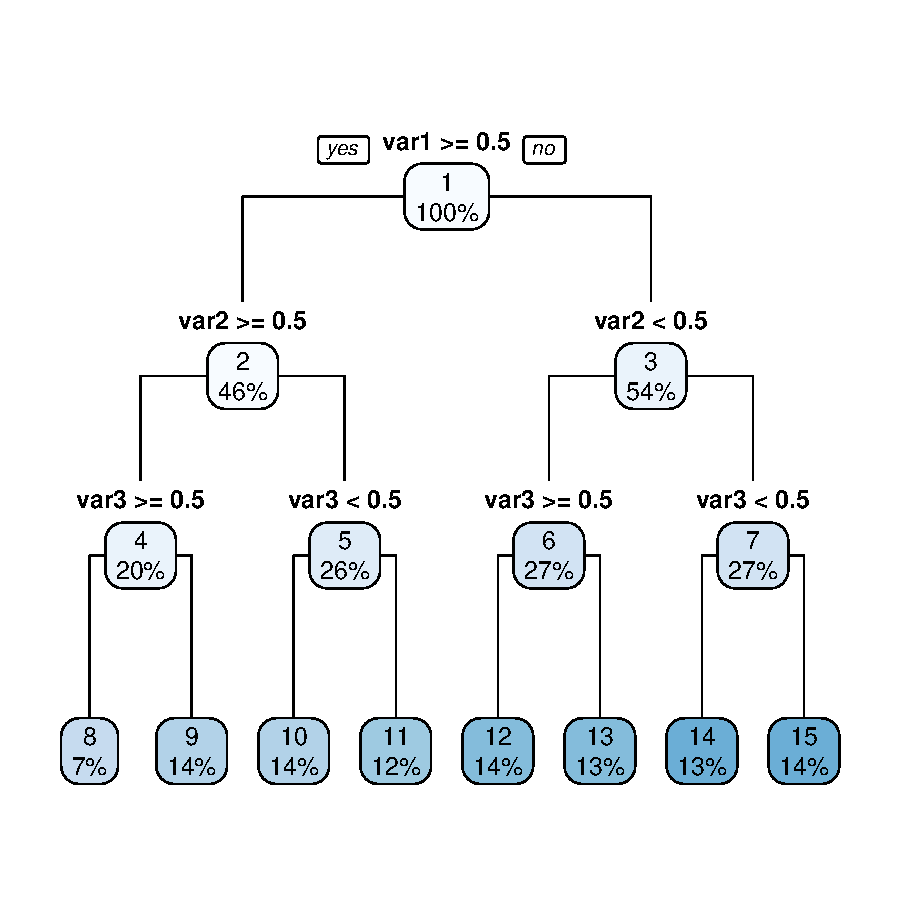
\includegraphics[width=.9\textwidth]{../../graphs/graph_tree_numeric.pdf}
\end{minipage}
\hfill
\begin{minipage}{0.48\textwidth}
    \captionof{figure}{CART (modified)}
    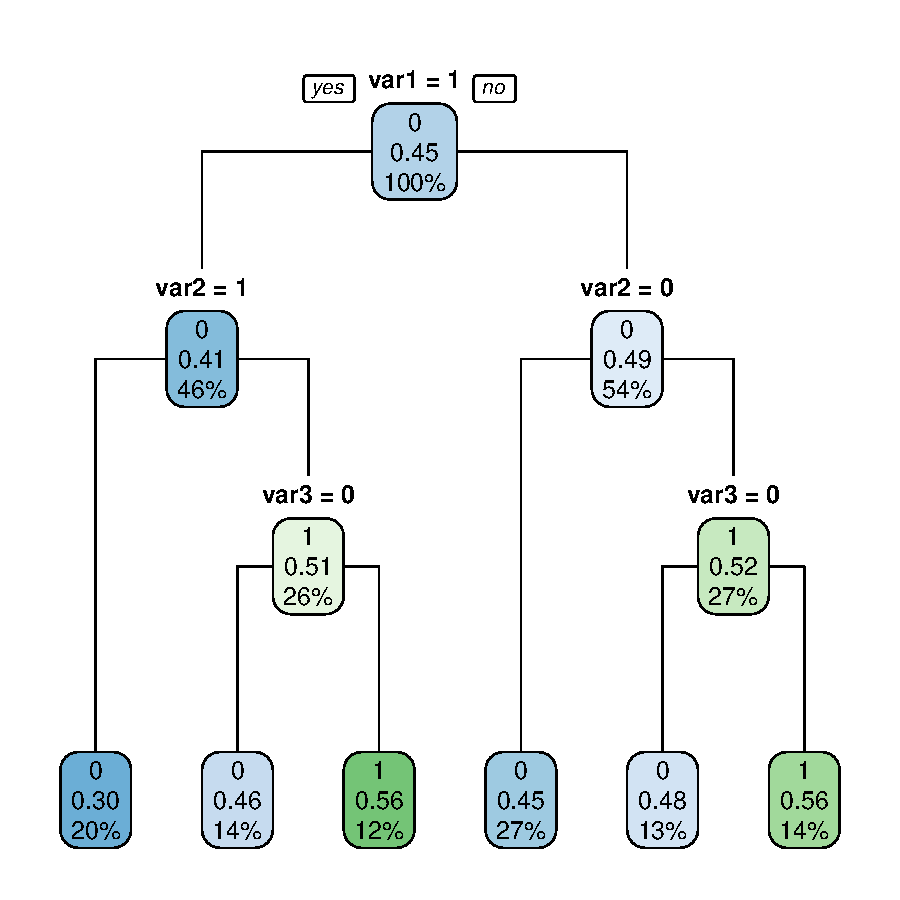
\includegraphics[width=.9\textwidth]{../../graphs/graph_tree_categorical.pdf}
\end{minipage}
}


\frame{\frametitle{Compare histogram x 100 synthetic datasets}
\begin{minipage}{0.48\textwidth}
    \captionof{figure}{CART (default)}
    \resizebox{\textwidth}{!}{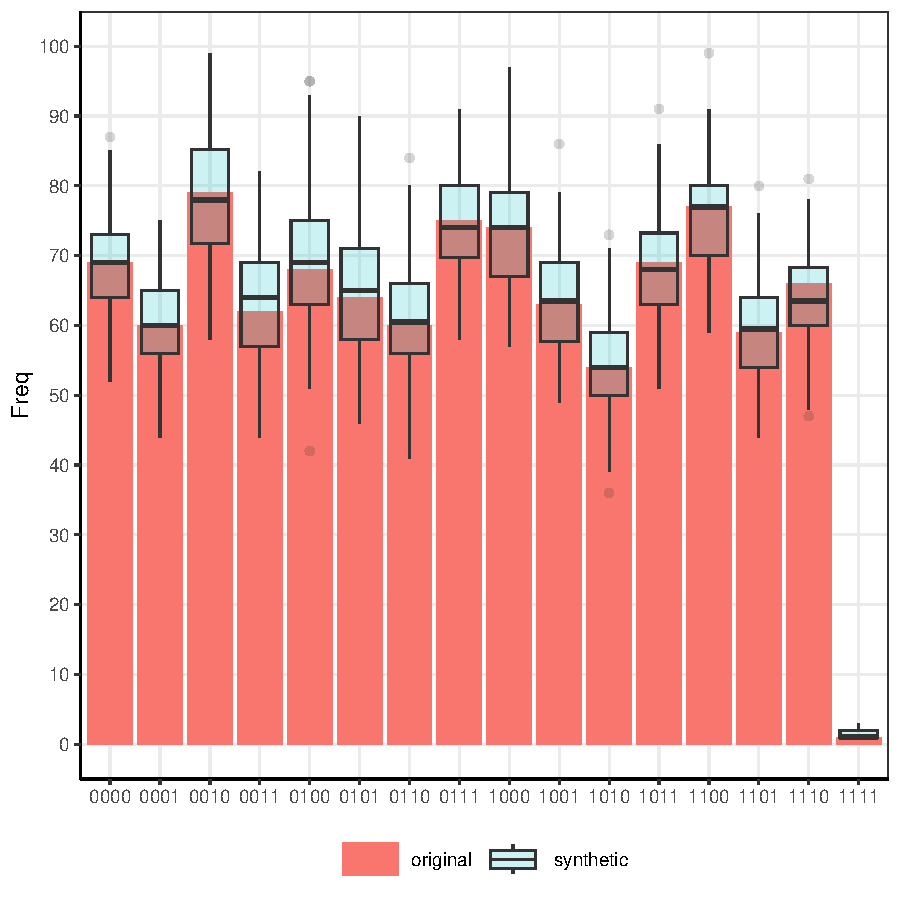
\includegraphics{../../graphs/graph_numeric_compare_histogram_100_v2.pdf}}
    \label{fig:graph_numeric_compare_histogram_100}
\end{minipage}
\hfill
\begin{minipage}{0.48\textwidth}
    \captionof{figure}{CART (modified)}
    \resizebox{\textwidth}{!}{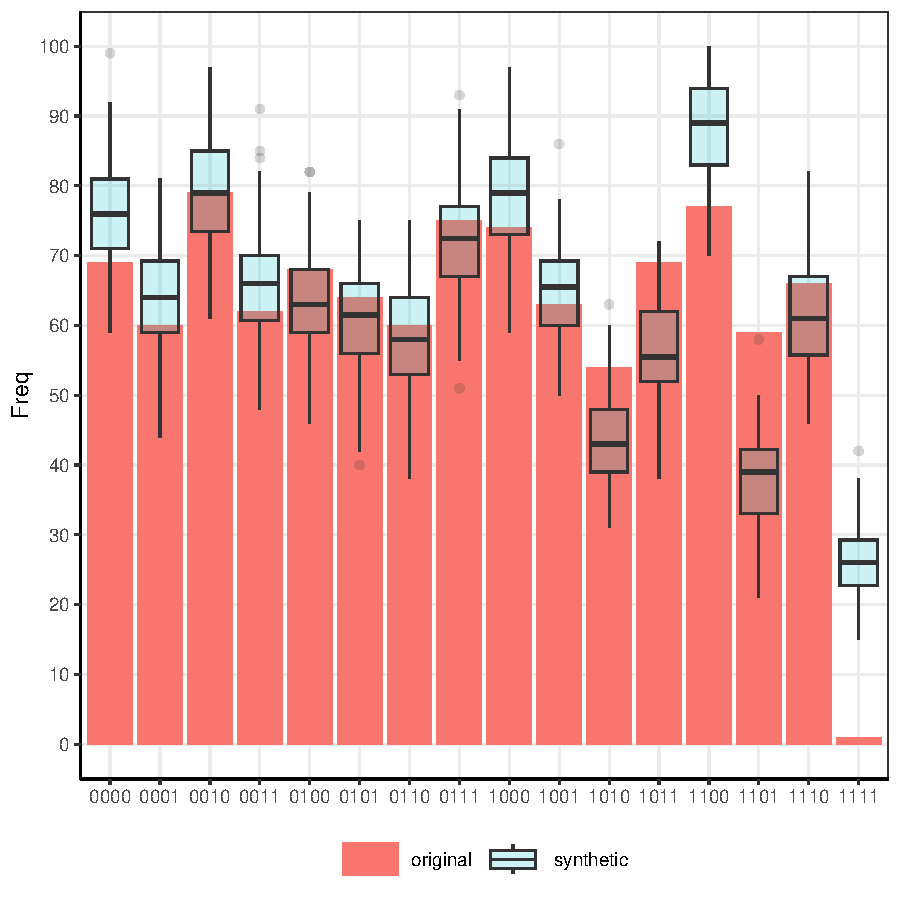
\includegraphics{../../graphs/graph_categorical_compare_histogram_100_v2.pdf}}
    \label{fig:graph_categorical_compare_histogram_100}
\end{minipage}

}


%%%%%%%%%%%%%%%%%%%%%%%%%%%%%%%%%%%%%%%%
%%%%%%%%%%%%%%%%%%%%%%%%%%%%%%%%%%%%%%%%
\section{Conclusion}\label{sec:conclusion}
%%%%%%%%%%%%%%%%%%%%%%%%%%%%%%%%%%%%%%%%
%%%%%%%%%%%%%%%%%%%%%%%%%%%%%%%%%%%%%%%%
\begin{frame}[c,plain]
\vskip-4mm
\begin{beamercolorbox}[wd=\boxwidth,ht=22.11mm]{transparent}%
    \vfill%
    \usebeamerfont{title}%
    \leftinsert%
    \MakeUppercase{Section \ref{sec:conclusion}: Conclusion} % <- Hier die Überschrift eintragen
\end{beamercolorbox}
\vskip-3mm
\pgfuseimage{rahmenlinie}
\end{frame}


\frame{\frametitle{Conclusion}
\begin{itemize}
    \item It has long been understood that there is a trade-off between utility and risk
    \item It seemed that CART models were less sensitive to this trade-off than other SDGs (i.e. higher utility, lower risk)
    \item Using a simulated data set, we show that CART models do not protect unique cases
    \item Using common privacy metrics, we show that these do not capture risk in our simulated data
    \begin{itemize}
        \item How do you know if there is a problem
    \end{itemize}
    \item It is possible to protect unique records, 
    \begin{itemize}
        \item You have to sacrifice utility
    \end{itemize}
    \item If you did not know there was a problem, why would you sacrifice utility?

\end{itemize}
}

\frame{\frametitle{Contact}
Jonathan Latner \\
\url{jonathan.latner@iab.de} \\

Reproducible code: 
\begin{itemize}
    \item Github: \url{https://github.com/jonlatner/KEM\_GAN/tree/main/latner/projects/simulation} 
\end{itemize}
}



\end{spacing}
\end{document}

